\documentclass[11pt]{article}

\usepackage[T1]{fontenc}
\usepackage[utf8]{inputenc}
\usepackage{lmodern}
\usepackage[a4paper,margin=28mm]{geometry}
\usepackage{microtype}
\usepackage{mathtools,amssymb,amsthm,bm}
\usepackage{booktabs,longtable,array}
\usepackage{enumitem}
\usepackage[dvipsnames]{xcolor}
\usepackage{graphicx}
\usepackage{float}
\usepackage{caption}
\usepackage{listings}
\usepackage{fancyhdr}
\usepackage{hyperref}
\usepackage[nameinlink,capitalise,noabbrev]{cleveref}

\hypersetup{
  colorlinks=true,
  linkcolor=MidnightBlue,
  citecolor=BrickRed,
  urlcolor=RoyalBlue,
  pdftitle={Exact Polynomial Windows from Finite Sums of Shifted and Scaled Rvachev up Functions},
  pdfauthor={Research report prepared for Vladimir Reshetnikov}
}
\urlstyle{same}

\pagestyle{fancy}
\fancyhf{}
\fancyhead[L]{Exact polynomial windows from Rvachev $\operatorname{up}$}
\fancyhead[R]{\thepage}
\renewcommand{\headrulewidth}{0.4pt}
\setlength{\headheight}{14pt}

\setlist[itemize]{leftmargin=1.7em,itemsep=0.25em,topsep=0.35em}
\setlist[enumerate]{leftmargin=1.9em,itemsep=0.3em,topsep=0.35em}
\setlength{\parindent}{1.2em}
\setlength{\parskip}{0.15em}
\allowdisplaybreaks

\newtheorem{theorem}{Theorem}[section]
\newtheorem{proposition}[theorem]{Proposition}
\newtheorem{corollary}[theorem]{Corollary}
\newtheorem{lemma}[theorem]{Lemma}
\newtheorem{conjecture}[theorem]{Conjecture}
\newtheorem{problem}[theorem]{Problem}
\theoremstyle{definition}
\newtheorem{definition}[theorem]{Definition}
\newtheorem{algorithm}[theorem]{Algorithm}
\theoremstyle{remark}
\newtheorem{remark}[theorem]{Remark}
\newtheorem{observation}[theorem]{Observation}

\DeclareMathOperator{\Up}{up}
\DeclareMathOperator{\supp}{supp}
\DeclareMathOperator{\ord}{ord}
\DeclareMathOperator{\spanop}{span}
\DeclareMathOperator{\diag}{diag}
\newcommand{\sinc}{\operatorname{sinc}}
\newcommand{\N}{\mathbb{N}}
\newcommand{\Z}{\mathbb{Z}}
\newcommand{\R}{\mathbb{R}}
\newcommand{\Q}{\mathbb{Q}}
\newcommand{\Pp}{\mathcal{P}}
\newcommand{\E}{\mathbb{E}}
\newcommand{\1}{\mathbf{1}}
\newcommand{\dd}{\,\mathrm{d}}
\newcommand{\e}{\mathrm{e}}
\newcommand{\BigO}{\mathcal{O}}
\newcommand{\CorpusNew}{\textcolor{ForestGreen}{\textsf{corpus-new}}}
\newcommand{\Classical}{\textcolor{MidnightBlue}{\textsf{classical}}}
\newcommand{\ProvedHere}{\textcolor{BrickRed}{\textsf{proved here}}}
\newcommand{\Conjectural}{\textcolor{Purple}{\textsf{conjectural}}}

\lstdefinestyle{pythonstyle}{
  language=Python,
  basicstyle=\ttfamily\small,
  keywordstyle=\color{MidnightBlue},
  commentstyle=\color{OliveGreen},
  stringstyle=\color{BrickRed},
  showstringspaces=false,
  breaklines=true,
  frame=single,
  columns=fullflexible
}

\title{\bfseries Exact Polynomial Windows from Finite Sums of Shifted and Scaled Rvachev $\operatorname{up}$ Functions\\[0.4em]
\large A constructive arbitrary-interval theory with binary partitions, Appell transforms, and support--sparsity tradeoffs}
\author{Research report prepared for Vladimir Reshetnikov}
\date{28 August 2026}

\begin{document}
\maketitle

\begin{abstract}
Let $u=\Up$ be the compactly supported $C^\infty$ Rvachev function, normalized by
$\supp u=[-1,1]$ and $\int u=1$.  This report gives a constructive answer to the
following local exact-representation problem: given a polynomial $p$ of degree at
most $d$ and a nondegenerate interval $[a,b]$, represent $p$ on the entire closed
interval as a \emph{finite} sum of shifted and scaled copies of $u$.

The central identity is an explicit locally finite formula for every repeated
left antiderivative of a scaled $u$ atom.  Its coefficients are restricted binary
partition numbers
\[
  p_m(N)=[z^N]\prod_{j=0}^{m-1}(1-z^{2^j})^{-1}.
\]
A support truncation converts that half-line identity into an exact finite formula
on $[a,b]$.  For an arbitrary scale parameter $h>0$, the construction uses
$(d+1)(1+\lceil(b-a)/(2h)\rceil)$ atoms.  In the sparse choice
$h=(b-a)/2$, every basis polynomial uses exactly two atoms; hence every
$p\in\Pp_d$ has a canonical representation with at most $2d+2$ raw $u$ atoms.
The coefficients are computed exactly by applying the reciprocal moment-generating
operator $M(D)^{-1}$, whose exponential coefficients are complete Bell polynomials
in Bernoulli-number cumulants of the $u$ distribution.

Further results include a monic Appell basis, a closed Wronskian and interpolation
determinant, an exact compactly supported $C^\infty$ extension operator, a
support--atom Pareto law, a Thue--Morse Green-function interpretation of the binary
weights, rationality and covariance properties, and numerical conditioning
analysis.  The report explicitly separates classical prior existence results of
V.~L. and V.~A. Rvachev from formulas that appear absent from the reviewed
\texttt{ProveIt} corpus.  Worldwide priority is not asserted for those formulas.
A fully commented Python implementation performs exact symbolic construction and
an independent sinc-product Fourier check.
\end{abstract}

\noindent\fbox{\parbox{0.965\textwidth}{
\textbf{Status convention.}
\Classical\ marks material already present in the literature or the repository;
\ProvedHere\ marks statements proved in this report;
\CorpusNew\ means that the statement was not found in the recursively reviewed
LaTeX corpus, not that worldwide novelty has been established;
\Conjectural\ marks unproved proposals.
}}

\tableofcontents
\newpage

\section{Executive summary}

The main conclusions are as follows.

\begin{enumerate}
\item \textbf{Exactness is possible only locally, but it is completely constructive.}
A nonzero polynomial cannot equal a finite compactly supported sum on all of
$\R$.  On any prescribed compact interval, however, an exact identity exists.

\item \textbf{One antiderivative generates a dyadic train.}
If
\[
  (Jf)(x)=\int_{-\infty}^{x}f(t)\dd t,
\]
then
\[
  Ju(x)=\sum_{k\geq0}u\!\left(\frac{x-(2k+1)}2\right),
\]
with a locally finite sum.  Iterating this identity produces restricted binary
partition numbers.

\item \textbf{Repeated antiderivatives have polynomial tails.}
If $Z$ has density $u$ and
\[
  A_n(y)=\E (y-Z)^n,
\]
then $A_n$ is a monic Appell polynomial and, beyond the support of an atom,
$J^{n+1}$ of that atom equals a constant multiple of $A_n$.

\item \textbf{Finite truncation is exact on an interval.}
With $L=b-a$, $h>0$, and $K=\lceil L/(2h)\rceil$, define
\[
\Psi_{n,h}^{[a,b]}(x)
 =n!2^{n(n+1)/2}\sum_{N=0}^{K}p_{n+1}(N)
 u\!\left(
 \frac{x-a-h(2^{n+1}-2+2N)}{2^{n+1}h}
 \right).
\]
Then, for every $x\in[a,b]$,
\[
  \Psi_{n,h}^{[a,b]}(x)
  =A_n\!\left(\frac{x-a+h}{h}\right).
\]
Consequently $\{\Psi_{0,h},\ldots,\Psi_{d,h}\}$ is a basis of $\Pp_d$ on the
interval.

\item \textbf{Two atoms per degree suffice.}
For $h=L/2$ one has $K=1$ and $p_m(0)=p_m(1)=1$.  Thus
\[
\Psi_n^{[a,b]}(x)=n!2^{n(n+1)/2}
\left[
 u\!\left(\frac{x-a-(2^n-1)L}{2^nL}\right)
 +u\!\left(\frac{x-a-2^nL}{2^nL}\right)
\right]
\]
equals $A_n(1+2(x-a)/L)$ on $[a,b]$.  A degree-$d$ polynomial therefore uses
at most $2d+2$ atoms.

\item \textbf{The coefficients are explicit.}
Let $c=a-h$, $\widetilde p(y)=p(c+hy)$, and
\[
 M(t)=\E\e^{tZ}=\prod_{j\geq1}\frac{\sinh(t/2^j)}{t/2^j},
 \qquad
 \frac1{M(t)}=\sum_{r\geq0}\gamma_r\frac{t^r}{r!}.
\]
Then
\[
 p(x)=\sum_{n=0}^{d}b_n\Psi_{n,h}^{[a,b]}(x),\qquad
 b_n=\sum_{r=0}^{d-n}
 \frac{\gamma_r h^{n+r}}{n!\,r!}\,p^{(n+r)}(c).
\]
All quantities are rational when the input data are rational.

\item \textbf{Support can be traded for atom count.}
The construction is supported in
\[
 [a-2h,\;a+h(2^{d+2}-2+2K)].
\]
Smaller $h$ gives a tighter collar but more atoms.  In particular, any requested
right collar $\rho>0$ is achieved by $h=\rho/2^{d+2}$ using at most
\[
 (d+1)\left(1+\left\lceil\frac{2^{d+1}L}{\rho}\right\rceil\right)
\]
atoms.

\item \textbf{Thue--Morse enters as a discrete inverse.}
The finite Thue--Morse polynomial
\[
 T_m(z)=\prod_{j=0}^{m-1}(1-z^{2^j})
       =\sum_{r=0}^{2^m-1}(-1)^{s_2(r)}z^r
\]
has $\{p_m(N)\}$ as its causal convolution inverse.  Thus the representation
weights are Green coefficients for a Thue--Morse finite-difference operator.
\end{enumerate}

\section{Scope, corpus audit, and prior art}

\subsection{Recursive repository audit}

The requested source tree was
\begin{center}
\url{https://github.com/VladimirReshetnikov/ProveIt/tree/main/Analysis/FabiusFunction/docs}.
\end{center}
The recursive audit used the repository's own ``second wave'' inventory as a
path-completeness check.  At the reviewed revision that inventory counted 67
LaTeX paths, grouped as shown in \cref{tab:corpus}.

\begin{table}[H]
\centering
\caption{Organization of the recursively reviewed LaTeX corpus.}
\label{tab:corpus}
\begin{tabular}{@{}lrp{0.57\textwidth}@{}}
\toprule
Class & Count & Role in the audit \\
\midrule
Living syntheses and references & 5 & Current definitions, notation, global identities, glossary, and audit metadata.\\
Frozen historical documents & 32 & Earlier reports and derivations, used to detect rediscovery and changes of notation.\\
Active frontier drafts & 23 & Representation, inverse, integration, transform, $q$-series, Thue--Morse, and Fourier-decay investigations; 12 are Fourier-decay dossiers.\\
Transcribed or corrected papers & 7 & Literature-facing source material and historical comparison.\\
\midrule
Total & 67 & All paths were included in the recursive search and thematic comparison.\\
\bottomrule
\end{tabular}
\end{table}

The closest internal sources were the representation syntheses
\texttt{Representation\_Frontiers.tex} and
\texttt{Representation\_Second\_Wave.tex}; the repeated-integration and
integral-transform drafts; the Appell/Bell-polynomial material; the finite and
infinite sinc-product studies; and the Thue--Morse/$q$-series files.  The corpus
already contains, among much else,

\begin{itemize}
\item the relation between the Fabius and Rvachev functions;
\item the refinement differential equation and infinite box-convolution model;
\item the probability law, moments, cumulants, and Bell-polynomial formulas;
\item Fourier products and the integer zero multiplicities $1+v_2(m)$;
\item dyadic Taylor/Appell blocks for the Fabius function;
\item repeated integration as a route from finite box splines to $u$;
\item many representation formulas for $u$, the Fabius function, and their
  transforms.
\end{itemize}

No formula equivalent to the interval basis in \cref{thm:finite-window}, the
binary-partition antiderivative identity in \cref{thm:iterated-J}, or the
coefficient transform in \cref{thm:coefficient-transform} was found in the
reviewed corpus.  This is the meaning of \CorpusNew\ below.

\subsection{Classical polynomial-representation results}

It would be incorrect to claim that polynomial representation by atomic
functions is new in itself.  The 1990 survey of V.~A. Rvachev states that the
spaces denoted there by $UP_n$ contain all polynomials of degree at most $n$ and
cites the 1972 paper of V.~L. Rvachev and V.~A. Rvachev, ``On the representation
of polynomials by functions with compact support'' \cite{RvachevRvachev1972,Rvachev1990}.
The survey also develops generalized Taylor systems made from finite-function
shifts.

The contribution attempted here is narrower and more explicit:

\begin{itemize}
\item a closed arbitrary-interval formula expressed only through shifted and
  scaled copies of the single function $u$;
\item a locally finite repeated-antiderivative identity with coefficients
  $p_m(N)$;
\item an immediately implementable exact coefficient transform;
\item the linear upper bound $2d+2$ in a canonical sparse construction;
\item exact support bounds and a tunable collar--atom tradeoff;
\item a Thue--Morse Green-function interpretation;
\item closed Wronskian and interpolation determinants;
\item a reproducible symbolic and numerical algorithm.
\end{itemize}

These formulas are presented as \ProvedHere\ and \CorpusNew, while worldwide
priority remains open pending a more exhaustive multilingual search of the
atomic-function literature.

\section{Normalization and basic facts}

\begin{definition}[Rvachev $u=\Up$]
Throughout, $u:\R\to\R$ denotes the unique normalized compactly supported
$C^\infty$ function satisfying
\begin{align}
 \supp u&=[-1,1], & u(x)&=u(-x), & \int_{\R}u(x)\dd x&=1,\label{eq:normalization}\\
 u'(x)&=2u(2x+1)-2u(2x-1).\label{eq:refinement-derivative}
\end{align}
The associated Fabius function satisfies $F(x)=u(x-1)$ on $[0,1]$ and
$u(x)=F(1-|x|)$ for $|x|\leq1$.
\end{definition}

A useful probability realization is
\begin{equation}
 Z=\sum_{j=1}^{\infty}2^{-j}V_j,
 \qquad V_j\stackrel{\mathrm{iid}}{\sim}\operatorname{Unif}[-1,1],
 \label{eq:random-Z}
\end{equation}
with density $u$.  Consequently
\begin{align}
 \widehat u(\xi)
 &=\E\e^{-i\xi Z}
 =\prod_{j=1}^{\infty}\sinc\!\left(\frac{\xi}{2^j}\right),
 &\sinc z&=\frac{\sin z}{z},\label{eq:fourier-product}\\
 M(t)
 &=\E\e^{tZ}
 =\prod_{j=1}^{\infty}\frac{\sinh(t/2^j)}{t/2^j}.
 \label{eq:mgf}
\end{align}
The variance is $\mu_2=1/9$.  The first even moments are
\begin{equation}
 \mu_0=1,\quad
 \mu_2=\frac19,\quad
 \mu_4=\frac{19}{675},\quad
 \mu_6=\frac{583}{59535},\quad
 \mu_8=\frac{132809}{32531625}.
 \label{eq:moments-first}
\end{equation}

\begin{lemma}[Strict one-sided monotonicity]
The function $u$ is strictly increasing on $(-1,0)$ and strictly decreasing on
$(0,1)$.
\end{lemma}

\begin{proof}
For $-1<x<0$, the term $u(2x-1)$ vanishes while $2x+1\in(-1,1)$ and
$u(2x+1)>0$, so \eqref{eq:refinement-derivative} gives $u'(x)>0$.  The case
$0<x<1$ follows symmetrically.  Positivity in the open support follows, for
example, from the infinite convolution model \eqref{eq:random-Z}.
\end{proof}

In particular, one atom cannot equal a nonzero constant on a nondegenerate
interval.  At least two atoms are required even in degree zero.

\section{The antiderivative train}

Let
\begin{equation}
 (Jf)(x)=\int_{-\infty}^{x}f(t)\dd t.
 \label{eq:J}
\end{equation}
The following elementary identity drives the entire construction.

\begin{proposition}[One-step antiderivative identity \ProvedHere, \CorpusNew]
\label{prop:one-step}
For every $x\in\R$,
\begin{equation}
 Ju(x)=\sum_{k=0}^{\infty}
 u\!\left(\frac{x-(2k+1)}{2}\right),
 \label{eq:one-step}
\end{equation}
where the sum is locally finite.
\end{proposition}

\begin{proof}
The $k$th summand is supported on $[2k-1,2k+3]$, so only finitely many terms
are nonzero at a fixed $x$.  Differentiating and using
\eqref{eq:refinement-derivative},
\begin{align*}
 \frac{\dd}{\dd x}u\!\left(\frac{x-(2k+1)}2\right)
 &=\frac12u'\!\left(\frac{x-(2k+1)}2\right)\\
 &=u(x-2k)-u(x-2k-2).
\end{align*}
The locally finite series telescopes to $u(x)$.  Both sides vanish for
sufficiently negative $x$, so the integration constant is zero.
\end{proof}

For a scale $h>0$ and center $c$, write
\begin{equation}
 u_{h,c}(x)=u\!\left(\frac{x-c}{h}\right).
 \label{eq:scaled-atom}
\end{equation}
Then \cref{prop:one-step} becomes
\begin{equation}
 J u_{h,c}(x)
 =h\sum_{k\geq0}
 u\!\left(\frac{x-c-h(2k+1)}{2h}\right).
 \label{eq:one-step-scaled}
\end{equation}

\subsection{Restricted binary partitions}

\begin{definition}
For $m\geq1$, let $p_m(N)$ be the restricted binary partition number
\begin{equation}
 p_m(N)=\#\left\{(k_0,\ldots,k_{m-1})\in\N^m:
 N=\sum_{j=0}^{m-1}2^jk_j\right\}.
 \label{eq:pm-def}
\end{equation}
Equivalently,
\begin{equation}
 \sum_{N\geq0}p_m(N)z^N
 =\prod_{j=0}^{m-1}\frac{1}{1-z^{2^j}}.
 \label{eq:pm-gf}
\end{equation}
\end{definition}

The first cases are
\[
 p_1(N)=1,
 \qquad
 p_2(N)=\left\lfloor\frac N2\right\rfloor+1,
\]
and the recurrence
\begin{equation}
 p_m(N)=p_{m-1}(N)+p_m(N-2^{m-1})
 \label{eq:pm-recurrence}
\end{equation}
holds with $p_m(N)=0$ for $N<0$.

\begin{theorem}[Repeated antiderivative formula \ProvedHere, \CorpusNew]
\label{thm:iterated-J}
For every integer $m\geq1$,
\begin{equation}
 J^m u_{h,c}(x)
 =h^m2^{m(m-1)/2}
 \sum_{N=0}^{\infty}p_m(N)
 u\!\left(
 \frac{x-c-h(2^m-1+2N)}{2^mh}
 \right).
 \label{eq:iterated-J}
\end{equation}
The sum is locally finite.
\end{theorem}

\begin{proof}
The case $m=1$ is \eqref{eq:one-step-scaled}.  Suppose the formula holds at
$m$.  Integrate each locally finite atom by \eqref{eq:one-step-scaled}.  An
atom with index $N$ has scale $2^mh$ and center
$c+h(2^m-1+2N)$, so a new index $k\geq0$ contributes scale $2^{m+1}h$ and
center
\begin{align*}
 &c+h(2^m-1+2N)+2^mh(2k+1)\\
 &\qquad=c+h\bigl(2^{m+1}-1+2(N+2^mk)\bigr).
\end{align*}
The prefactor is multiplied by $2^mh$, becoming
$h^{m+1}2^{m(m+1)/2}$.  The multiplicity of the new index $N'$ is
\[
 \sum_{k\geq0}p_m(N'-2^mk)=p_{m+1}(N'),
\]
which is exactly \eqref{eq:pm-recurrence}.  This proves the induction.

For local finiteness, the atom indexed by $N$ has left support endpoint
computed in \cref{cor:support-edge}; this endpoint tends to $+\infty$ with
$N$.
\end{proof}

\begin{corollary}[Support-edge invariance \ProvedHere, \CorpusNew]
\label{cor:support-edge}
The $N$th atom on the right side of \eqref{eq:iterated-J} has support
\begin{equation}
 \left[c-h+2hN,\;c+h(2^{m+1}-1+2N)\right].
 \label{eq:atom-support-general}
\end{equation}
In particular, its \emph{left} endpoint $c-h+2hN$ is independent of the
antiderivative order $m$.
\end{corollary}

This invariance is the geometric reason a single truncation index can be used
simultaneously for every polynomial degree.

\subsection{Thue--Morse as the inverse difference operator}

Let $s_2(r)$ denote the binary digit sum and
$\varepsilon_r=(-1)^{s_2(r)}$.  The finite Prouhet--Thue--Morse polynomial is
\begin{equation}
 T_m(z)=\prod_{j=0}^{m-1}(1-z^{2^j})
 =\sum_{r=0}^{2^m-1}\varepsilon_r z^r.
 \label{eq:Tm}
\end{equation}

\begin{proposition}[Thue--Morse Green sequence \ProvedHere, \CorpusNew]
\label{prop:tm-green}
The restricted binary partition sequence is the causal convolution inverse of
the length-$2^m$ signed Thue--Morse block:
\begin{equation}
 \sum_{r=0}^{\min(N,2^m-1)}
 (-1)^{s_2(r)}p_m(N-r)=\delta_{N0}.
 \label{eq:tm-inverse}
\end{equation}
Equivalently, if $S$ is the backward shift on sequences, then
\begin{equation}
 \left[\prod_{j=0}^{m-1}(I-S^{2^j})\right]p_m=\delta_0.
 \label{eq:tm-green-operator}
\end{equation}
\end{proposition}

\begin{proof}
Multiply the generating functions \eqref{eq:pm-gf} and \eqref{eq:Tm}.
Their product is one.  Coefficient extraction gives \eqref{eq:tm-inverse},
and the shift-operator form is the same convolution identity.
\end{proof}

Thus the continuous inverse of the refinement derivative and the discrete
inverse of a Thue--Morse difference stencil appear in the same formula.  This
is more than a decorative analogy: the weights in the exact polynomial window
are the Green coefficients that undo all $m$ dyadic differences.

\begin{proposition}[Quasipolynomial structure \ProvedHere]
\label{prop:pm-quasi}
For fixed $m$, $p_m(N)$ is a quasipolynomial in $N$ of degree $m-1$ and period
dividing $2^{m-1}$.  Its leading term is independent of the residue class:
\begin{equation}
 p_m(N)=\frac{N^{m-1}}
 {(m-1)!\,2^{m(m-1)/2}}+\BigO(N^{m-2}).
 \label{eq:pm-asymptotic}
\end{equation}
Consequently, for $m=n+1$ the normalized weight
\begin{equation}
 w_{n,N}=n!2^{n(n+1)/2}p_{n+1}(N)
 \label{eq:normalized-weight}
\end{equation}
is a monic degree-$n$ quasipolynomial:
$w_{n,N}=N^n+\BigO(N^{n-1})$.
\end{proposition}

\begin{proof}
The generating function \eqref{eq:pm-gf} is rational and all its poles are
$2^{m-1}$th roots of unity.  Partial fractions therefore give a finite sum of
polynomial multiples of root-of-unity exponentials, hence a quasipolynomial
with period dividing $2^{m-1}$.  The pole at $z=1$ has order $m$.  Since
\[
 1-z^{2^j}=2^j(1-z)+\BigO((1-z)^2),
\]
we have
\[
 \prod_{j=0}^{m-1}(1-z^{2^j})
 =2^{m(m-1)/2}(1-z)^m(1+\BigO(1-z)).
\]
The coefficient of $(1-z)^{-m}$ is
$\binom{N+m-1}{m-1}$, giving \eqref{eq:pm-asymptotic}.
\end{proof}

\section{Polynomial tails and the $u$-Appell family}

\begin{definition}
Let $Z$ have density $u$.  Define
\begin{equation}
 A_n(y)=\E (y-Z)^n.
 \label{eq:An-def}
\end{equation}
By symmetry of $Z$, this is also $\E(y+Z)^n$.
\end{definition}

\begin{proposition}[Appell structure \Classical/\ProvedHere]
\label{prop:appell}
The polynomials $A_n$ are monic and satisfy
\begin{align}
 \sum_{n=0}^{\infty}A_n(y)\frac{t^n}{n!}
 &=\e^{yt}M(t),\label{eq:An-egf}\\
 A_n'(y)&=nA_{n-1}(y),\label{eq:An-appell}\\
 A_n(y)&=\sum_{r=0}^{n}\binom nr\mu_r y^{n-r}.
 \label{eq:An-moments}
\end{align}
\end{proposition}

\begin{proof}
Take expectations in $\e^{t(y-Z)}$.  Symmetry gives
$\E\e^{-tZ}=M(t)$.  Expanding the exponential gives
\eqref{eq:An-egf}; differentiation and coefficient extraction give the other
identities.
\end{proof}

The first members are
\begin{align*}
 A_0(y)&=1,\\
 A_1(y)&=y,\\
 A_2(y)&=y^2+\frac19,\\
 A_3(y)&=y^3+\frac13y,\\
 A_4(y)&=y^4+\frac23y^2+\frac{19}{675},\\
 A_5(y)&=y^5+\frac{10}{9}y^3+\frac{19}{135}y,\\
 A_6(y)&=y^6+\frac53y^4+\frac{19}{45}y^2+\frac{583}{59535}.
\end{align*}

\begin{theorem}[Tail-polynomial identity \ProvedHere]
\label{thm:tail-polynomial}
For $n\geq0$ and $x\geq c+h$,
\begin{equation}
 J^{n+1}u_{h,c}(x)
 =\frac{h^{n+1}}{n!}
 A_n\!\left(\frac{x-c}{h}\right).
 \label{eq:tail-polynomial}
\end{equation}
\end{theorem}

\begin{proof}
Repeated integration gives the standard truncated-power kernel
\[
 J^{n+1}u_{h,c}(x)
 =\frac1{n!}\int_{-\infty}^{x}(x-t)^n
 u\!\left(\frac{t-c}{h}\right)\dd t.
\]
For $x\geq c+h$, the full support $[c-h,c+h]$ lies below $x$.  Substitute
$t=c+hz$ to obtain
\[
 \frac{h^{n+1}}{n!}
 \int_{-1}^{1}\left(\frac{x-c}{h}-z\right)^nu(z)\dd z,
\]
which is \eqref{eq:tail-polynomial}.
\end{proof}

Combining \cref{thm:iterated-J,thm:tail-polynomial} yields a locally finite
half-line representation that is already of independent interest.

\begin{corollary}[Half-line polynomial identity \ProvedHere, \CorpusNew]
\label{cor:halfline}
For $x\geq c+h$,
\begin{equation}
 A_n\!\left(\frac{x-c}{h}\right)
 =n!2^{n(n+1)/2}\sum_{N\geq0}p_{n+1}(N)
 u\!\left(
 \frac{x-c-h(2^{n+1}-1+2N)}{2^{n+1}h}
 \right).
 \label{eq:halfline}
\end{equation}
The right side is locally finite.
\end{corollary}

\section{The exact finite-window theorem}

We now truncate the half-line train using the support-edge invariance.

\begin{theorem}[Exact finite polynomial window \ProvedHere, \CorpusNew]
\label{thm:finite-window}
Let $a<b$, $h>0$, $L=b-a$, and
\begin{equation}
 K=\left\lceil\frac{L}{2h}\right\rceil.
 \label{eq:K}
\end{equation}
For every $n\geq0$, define
\begin{equation}
\boxed{
\begin{aligned}
 \Psi_{n,h}^{[a,b]}(x)
 &=n!2^{n(n+1)/2}\sum_{N=0}^{K}p_{n+1}(N)\\[-0.2em]
 &\quad\times
 u\!\left(
 \frac{x-a-h(2^{n+1}-2+2N)}{2^{n+1}h}
 \right).
\end{aligned}}
\label{eq:Psi-general}
\end{equation}
Then on the full closed interval $[a,b]$,
\begin{equation}
 \Psi_{n,h}^{[a,b]}(x)
 =A_n\!\left(\frac{x-a+h}{h}\right).
 \label{eq:Psi-Appell}
\end{equation}
Consequently, for every $d\geq0$,
\begin{equation}
 \spanop\{\Psi_{0,h}^{[a,b]},\ldots,
 \Psi_{d,h}^{[a,b]}\}\big|_{[a,b]}=\Pp_d.
 \label{eq:basis-Pd}
\end{equation}
\end{theorem}

\begin{proof}
Set $c=a-h$.  Then $x\geq a=c+h$ throughout the interval, so
\cref{cor:halfline} applies and its atom centers become
\[
 c+h(2^{n+1}-1+2N)
 =a+h(2^{n+1}-2+2N).
\]
By \cref{cor:support-edge}, the left endpoint of the atom indexed by $N$ is
\[
 c-h+2hN=a-2h+2hN.
\]
For every omitted index $N\geq K+1$, this endpoint satisfies
\[
 a-2h+2hN\geq a+2hK\geq b.
\]
Thus every omitted atom vanishes on $[a,b]$; at a possible equality $x=b$,
its argument is $-1$ and $u(-1)=0$.  The finite truncation therefore agrees
exactly with the full half-line identity, proving \eqref{eq:Psi-Appell}.
Since $A_n$ is monic of degree $n$, the displayed family is a polynomial basis.
\end{proof}

\begin{remark}[Why the interval is essential]
Every finite sum in \eqref{eq:Psi-general} is compactly supported.  A nonzero
polynomial is not compactly supported, so a global identity on all of $\R$ is
impossible.  The theorem constructs an exact \emph{window}: polynomial on the
specified interval, smoothly transitioning elsewhere, and identically zero
outside a finite support.
\end{remark}

\subsection{Two atoms per degree}

\begin{corollary}[Sparse two-atom basis \ProvedHere, \CorpusNew]
\label{cor:two-atom}
If $h\geq L/2$, then $K=1$ and
\begin{equation}
\begin{aligned}
 \Psi_{n,h}^{[a,b]}(x)
 =n!2^{n(n+1)/2}\bigg[&
 u\!\left(\frac{x-a-h(2^{n+1}-2)}{2^{n+1}h}\right)\\
 &+u\!\left(\frac{x-a-h2^{n+1}}{2^{n+1}h}\right)
 \bigg].
 \label{eq:two-atom-general-h}
\end{aligned}
\end{equation}
It equals $A_n((x-a+h)/h)$ on $[a,b]$.
\end{corollary}

\begin{proof}
Since $L/(2h)\in(0,1]$, its ceiling is one.  Also
$p_m(0)=p_m(1)=1$ for all $m\geq1$.
\end{proof}

The smallest support within this sparse causal family is obtained at
$h=L/2$.

\begin{corollary}[Canonical interval formula \ProvedHere, \CorpusNew]
\label{cor:canonical}
Let $L=b-a$.  Define
\begin{equation}
\boxed{
\begin{aligned}
 \Psi_n^{[a,b]}(x)
 =n!2^{n(n+1)/2}\bigg[&
 u\!\left(\frac{x-a-(2^n-1)L}{2^nL}\right)\\
 &+u\!\left(\frac{x-a-2^nL}{2^nL}\right)
 \bigg].
\end{aligned}}
\label{eq:canonical-Psi}
\end{equation}
Then
\begin{equation}
 \Psi_n^{[a,b]}(x)=A_n\!\left(1+\frac{2(x-a)}L\right),
 \qquad a\leq x\leq b.
 \label{eq:canonical-Appell}
\end{equation}
Every polynomial of degree at most $d$ has a representation using at most
$2d+2$ raw $u$ atoms.
\end{corollary}

For $n=0$, \eqref{eq:canonical-Psi} reduces to the familiar partition identity
\begin{equation}
 u\!\left(\frac{x-a}{L}\right)
 +u\!\left(\frac{x-b}{L}\right)=1,
 \qquad a\leq x\leq b.
 \label{eq:partition-unity-interval}
\end{equation}
The theorem can therefore be viewed as a complete higher-degree lift of the
basic two-shift partition of unity.

\section{Exact coefficient extraction}

The basis theorem becomes an algorithm once the polynomial is converted to the
Appell coordinates.

\subsection{Cumulants, Bernoulli numbers, and the reciprocal MGF}

Write
\begin{equation}
 \log M(t)=\sum_{r\geq1}\kappa_r\frac{t^r}{r!}.
 \label{eq:cumulant-def}
\end{equation}
From the product \eqref{eq:mgf} and the classical expansion of
$\log(\sinh z/z)$,
\begin{equation}
 \kappa_{2m}
 =\frac{2^{2m-1}B_{2m}}{m(2^{2m}-1)},
 \qquad
 \kappa_{2m+1}=0.
 \label{eq:cumulants}
\end{equation}
Define
\begin{equation}
 G(t)=\frac1{M(t)}
 =\sum_{r=0}^{\infty}\gamma_r\frac{t^r}{r!}.
 \label{eq:G-gamma}
\end{equation}
Then
\begin{equation}
 \gamma_r=Y_r(-\kappa_1,\ldots,-\kappa_r),
 \label{eq:gamma-Bell}
\end{equation}
where $Y_r$ is the complete exponential Bell polynomial.  Equivalently,
\begin{equation}
 \gamma_0=1,
 \qquad
 \gamma_n=-\sum_{r=1}^{n}\binom{n-1}{r-1}
 \kappa_r\gamma_{n-r}.
 \label{eq:gamma-recurrence}
\end{equation}
The first values are
\begin{align}
 \gamma_0&=1,&
 \gamma_2&=-\frac19,&
 \gamma_4&=\frac{31}{675},\nonumber\\
 \gamma_6&=-\frac{2347}{59535},&
 \gamma_8&=\frac{1904369}{32531625},&
 \gamma_{10}&=-\frac{3309760579}{24405225075},
 \label{eq:gamma-values}
\end{align}
with all odd coefficients zero.

\begin{theorem}[Coefficient transform \ProvedHere, \CorpusNew]
\label{thm:coefficient-transform}
Let $p\in\Pp_d$, $c=a-h$, and
\begin{equation}
 \widetilde p(y)=p(c+hy).
 \label{eq:ptilde}
\end{equation}
There is a unique expansion
\begin{equation}
 \widetilde p(y)=\sum_{n=0}^{d}b_nA_n(y),
 \label{eq:Appell-expansion}
\end{equation}
and its coefficients are given by any of the equivalent formulas
\begin{align}
 q(y)&=G(D)\widetilde p(y)
 =\sum_{r=0}^{d}\frac{\gamma_r}{r!}\widetilde p^{(r)}(y),
 &b_n&=[y^n]q(y),\label{eq:q-transform}\\
 b_n&=\sum_{r=0}^{d-n}
 \frac{\gamma_r h^{n+r}}{n!\,r!}\,p^{(n+r)}(c),
 \label{eq:b-derivative}\\
 b_n&=\sum_{r=0}^{d-n}\binom{n+r}{r}\gamma_r c_{n+r}
 \quad\text{if}\quad
 \widetilde p(y)=\sum_{j=0}^{d}c_jy^j.
 \label{eq:b-coefficient}
\end{align}
Therefore
\begin{equation}
 p(x)=\sum_{n=0}^{d}b_n\Psi_{n,h}^{[a,b]}(x),
 \qquad x\in[a,b].
 \label{eq:p-Psi}
\end{equation}
\end{theorem}

\begin{proof}
The moment formula \eqref{eq:An-moments} says precisely that
\begin{equation}
 A_n(y)=M(D)y^n.
 \label{eq:MD}
\end{equation}
Since $M(0)=1$, the formal differential operator $M(D)$ is invertible on every
finite-dimensional polynomial space, with inverse $G(D)$.  Apply $G(D)$ to
\eqref{eq:Appell-expansion} to obtain
$q(y)=\sum b_ny^n$, proving \eqref{eq:q-transform}.  Taking the coefficient of
$y^n$, or equivalently the $n$th derivative at zero, gives
\eqref{eq:b-derivative}.  Direct coefficient extraction gives
\eqref{eq:b-coefficient}.  Finally use \eqref{eq:Psi-Appell}.
\end{proof}

The raw amplitude of the atom at level $n$ and partition index $N$ is therefore
\begin{equation}
 \alpha_{n,N}
 =n!2^{n(n+1)/2}b_n p_{n+1}(N).
 \label{eq:alpha-nN}
\end{equation}
In the sparse construction $N\in\{0,1\}$ and both atoms at level $n$ have the
same amplitude
\begin{equation}
 \alpha_n=n!2^{n(n+1)/2}b_n.
 \label{eq:alpha-n}
\end{equation}

\subsection{A triangular alternative}

If $\widetilde p(y)=\sum c_ny^n$, monicity of $A_n$ gives the descending
recurrence
\begin{equation}
 b_n=c_n-\sum_{k=n+1}^{d}b_k\binom{k}{n}\mu_{k-n},
 \qquad n=d,d-1,\ldots,0.
 \label{eq:triangular-b}
\end{equation}
This is often the simplest exact-rational implementation when the moments are
already available.

\subsection{Closed monomial coefficients}

Define the reciprocal Appell family
\begin{equation}
 C_m(y)=G(D)y^m
 =\sum_{r=0}^{m}\binom mr\gamma_r y^{m-r}.
 \label{eq:C-reciprocal-Appell}
\end{equation}
For $p(x)=(x-a)^m$, one has
\begin{equation}
 b_n=h^m\binom mn C_{m-n}(-1),
 \qquad 0\leq n\leq m.
 \label{eq:monomial-b}
\end{equation}
Thus all monomial windows admit a direct Bernoulli--Bell closed form with no
linear solve.

\section{Algorithm and arithmetic complexity}

\begin{algorithm}[Exact construction]
\label{alg:construction}
Input a polynomial $p(x)$ of degree $d$, a nondegenerate interval $[a,b]$, and
a scale $h>0$.

\begin{enumerate}
\item Set $L=b-a$, $c=a-h$, and $K=\lceil L/(2h)\rceil$.
\item Compute $\kappa_0,\ldots,\kappa_d$ from \eqref{eq:cumulants}.
\item Compute $\gamma_0,\ldots,\gamma_d$ by \eqref{eq:gamma-recurrence}.
\item Form $\widetilde p(y)=p(c+hy)$ and compute $b_n$ using
  \eqref{eq:b-derivative}, \eqref{eq:b-coefficient}, or
  \eqref{eq:triangular-b}.
\item Build the arrays $p_m(N)$, $1\leq m\leq d+1$, $0\leq N\leq K$, by the
  dynamic recurrence \eqref{eq:pm-recurrence}.
\item For each $0\leq n\leq d$ and $0\leq N\leq K$, emit the atom
\begin{align*}
 H_n&=2^{n+1}h,\\
 C_{n,N}&=a+h(2^{n+1}-2+2N),\\
 \alpha_{n,N}&=n!2^{n(n+1)/2}b_np_{n+1}(N).
\end{align*}
\item Return
\[
 \sum_{n=0}^{d}\sum_{N=0}^{K}
 \alpha_{n,N}u\!\left(\frac{x-C_{n,N}}{H_n}\right).
\]
\end{enumerate}
\end{algorithm}

If the partition arrays are updated incrementally in $m$, the arithmetic
operation count is
\begin{equation}
 \BigO(d^2+dK),
 \label{eq:complexity}
\end{equation}
not counting coefficient bit growth.  The output itself contains
$(d+1)(K+1)$ atoms, so the $dK$ term is unavoidable for an explicit atom list.
In the sparse case $K=1$, the output and construction are linear in $d$ after
the $\BigO(d^2)$ coefficient transform.

\section{Structural properties}

\subsection{Uniqueness in the block basis}

\begin{proposition}[Block-basis uniqueness]
For fixed $a,b,h,d$, the coefficients $b_0,\ldots,b_d$ in
\eqref{eq:p-Psi} are unique.
\end{proposition}

\begin{proof}
The restrictions of $\Psi_{n,h}$ are the monic degree-$n$ polynomials
$A_n((x-a+h)/h)$.  A triangular polynomial basis has unique coordinates.
\end{proof}

This does \emph{not} claim uniqueness if the amplitudes of all raw atoms are
allowed to vary independently.  The canonical object is the equal-amplitude
binary-partition block at each degree.

\subsection{Derivative ladder, Wronskian, and interpolation}

\begin{proposition}[Derivative ladder \ProvedHere]
For $0\leq k\leq n$ and $x\in[a,b]$,
\begin{equation}
 \frac{\dd^k}{\dd x^k}\Psi_{n,h}^{[a,b]}(x)
 =\frac{(n)_k}{h^k}\Psi_{n-k,h}^{[a,b]}(x),
 \label{eq:derivative-ladder}
\end{equation}
where $(n)_k=n(n-1)\cdots(n-k+1)$.
\end{proposition}

\begin{proof}
Differentiate \eqref{eq:Psi-Appell} and use the Appell relation
\eqref{eq:An-appell}.
\end{proof}

\begin{theorem}[Wronskian and interpolation determinant \ProvedHere, \CorpusNew]
\label{thm:determinants}
For every $x\in[a,b]$,
\begin{equation}
 W(\Psi_{0,h},\ldots,\Psi_{d,h})(x)
 =h^{-d(d+1)/2}\prod_{n=0}^{d}n!.
 \label{eq:Wronskian}
\end{equation}
For distinct nodes $x_0,\ldots,x_d\in[a,b]$,
\begin{equation}
 \det\bigl[\Psi_{j,h}(x_i)\bigr]_{i,j=0}^{d}
 =h^{-d(d+1)/2}\prod_{0\leq i<j\leq d}(x_j-x_i).
 \label{eq:interpolation-det}
\end{equation}
\end{theorem}

\begin{proof}
After the affine change $y=(x-a+h)/h$, the basis consists of monic polynomials
$A_j(y)$.  Changing from monomials to a monic triangular basis has determinant
one.  The monomial Wronskian is $\prod j!$, and each derivative row contributes
a factor $h^{-k}$.  The interpolation determinant is the ordinary Vandermonde
in the $y_i$ variables.
\end{proof}

Hence the block basis is an extended complete Chebyshev system on every
subinterval.  Polynomial interpolation in this basis is nonsingular at every
set of distinct nodes.

\subsection{Affine covariance and rationality}

The entire construction is affine-covariant.  If $x=\lambda X+\tau$ with
$\lambda>0$, centers and scales transform by the same affine map, while the
Appell coefficient transform is exactly the usual polynomial pullback.

If $p\in\Q[x]$ and $a,b,h\in\Q$ with $h>0$, then
\begin{itemize}
\item all moments, cumulants, and $\gamma_r$ are rational;
\item all $b_n$ and amplitudes $\alpha_{n,N}$ are rational;
\item every center and scale is rational, and all scale ratios are dyadic.
\end{itemize}
Thus the representation can be constructed without floating-point arithmetic.

\subsection{A compactly supported smooth extension operator}

For fixed $d,a,b,h$, define
\begin{equation}
 E_{d,a,b,h}p(x)=
 \sum_{n=0}^{d}\sum_{N=0}^{K}
 \alpha_{n,N}(p)
 u\!\left(\frac{x-C_{n,N}}{H_n}\right).
 \label{eq:extension-operator}
\end{equation}
Then $E_{d,a,b,h}:\Pp_d\to C_c^\infty(\R)$ is linear and injective, and
\begin{equation}
 (E_{d,a,b,h}p)(x)=p(x),\qquad x\in[a,b].
 \label{eq:restriction-right-inverse}
\end{equation}
All derivatives match on the closed interval.  Outside a finite support the
extension vanishes identically, with infinite-order flatness at its external
support endpoints inherited from $u$.

\subsection{A norm bound}

Since $0\leq u\leq1$, the global supremum norm satisfies
\begin{equation}
 \|E_{d,a,b,h}p\|_{\infty}
 \leq\sum_{n=0}^{d}|b_n|n!2^{n(n+1)/2}
 \sum_{N=0}^{K}p_{n+1}(N).
 \label{eq:norm-bound}
\end{equation}
This bound is crude but useful as a symbolic stability certificate.

\section{Support, sparsity, and localization}

The support of the $(n,N)$ atom in \eqref{eq:Psi-general} is
\begin{equation}
 [a-2h+2hN,\;a+h(2^{n+2}-2+2N)].
 \label{eq:support-nN}
\end{equation}
Therefore the full degree-$d$ construction is supported in
\begin{equation}
 \supp E_{d,a,b,h}p
 \subseteq
 [a-2h,\;a+h(2^{d+2}-2+2K)].
 \label{eq:support-total}
\end{equation}
Because $2hK<L+2h$,
\begin{equation}
 \sup\supp E_{d,a,b,h}p<b+2^{d+2}h.
 \label{eq:support-simple}
\end{equation}

\begin{theorem}[Collar--atom tradeoff \ProvedHere, \CorpusNew]
\label{thm:collar}
Let $\rho>0$ and choose
\begin{equation}
 h=\frac{\rho}{2^{d+2}}.
 \label{eq:h-collar}
\end{equation}
Then every $p\in\Pp_d$ has an exact $u$-atom representation on $[a,b]$
supported in $[a-\rho,b+\rho]$ and using at most
\begin{equation}
 (d+1)\left(
 1+\left\lceil\frac{2^{d+1}(b-a)}{\rho}\right\rceil
 \right)
 \label{eq:collar-count}
\end{equation}
atoms.
\end{theorem}

\begin{proof}
The left overhang is $2h=\rho/2^{d+1}\leq\rho$, and
\eqref{eq:support-simple} gives a right overhang less than $2^{d+2}h=\rho$.
The atom count is $(d+1)(K+1)$ with
$K=\lceil(b-a)/(2h)\rceil$.
\end{proof}

More generally, for asymmetric collars $\rho_-,\rho_+>0$, it is sufficient to
choose
\begin{equation}
 h\leq\min\left\{\frac{\rho_-}{2},
 \frac{\rho_+}{2^{d+2}}\right\}.
 \label{eq:asymmetric-h}
\end{equation}
A reflected, right-causal construction interchanges the two collar roles.

In the sparse choice $h=L/2$, the exact support bound is
\begin{equation}
 \supp E_{d,a,b,L/2}p
 \subseteq[a-L,\;a+2^{d+1}L].
 \label{eq:sparse-support}
\end{equation}
Thus linear atom count comes with an exponentially long one-sided scale ladder.
The general-$h$ theorem permits one to exchange that long tail for more atoms.

\section{Relation to shift-invariant reproduction}

A superficial reading might suggest a contradiction with the Strang--Fix
conditions.  There is none.

Under the Fourier convention \eqref{eq:fourier-product}, $\widehat u$ has a zero
at every nonzero $2\pi k$ of multiplicity
\begin{equation}
 1+v_2(k).
 \label{eq:zero-multiplicity}
\end{equation}
The minimum multiplicity is one, attained at odd $k$.  Hence the single
fixed-scale integer-shift space generated by $u$ has only first-order global
polynomial reproduction in the standard Strang--Fix sense: constants are the
uniformly reproduced polynomials, but a fixed lattice of one scale does not
globally reproduce arbitrary higher degrees \cite{StrangFix1973,deBoorRon1992}.

The present construction bypasses that obstruction in three simultaneous ways:

\begin{enumerate}
\item it asks for equality only on a bounded interval;
\item it is boundary-adapted and truncates atoms by support;
\item it uses a dyadic chain of scales $2^{n+1}h$ rather than one principal
  shift-invariant space.
\end{enumerate}

This viewpoint helps reconcile the classical $UP_n$ polynomial inclusion with
modern Fourier reproduction theory.  The exact window is a multiscale,
boundary-generated object, not a global cardinal reproduction formula.

\section{Worked exact example}

Take
\begin{equation}
 p(x)=3x^4-2x^3+5x-7,
 \qquad [a,b]=[0,1],
 \qquad h=\frac12.
 \label{eq:quartic}
\end{equation}
Then $c=-1/2$ and
\begin{equation}
 \widetilde p(y)=p\!\left(\frac{y-1}{2}\right)
 =\frac{3}{16}y^4-y^3+\frac{15}{8}y^2+y-\frac{145}{16}.
 \label{eq:quartic-tilde}
\end{equation}
The exact Appell coefficients are
\begin{equation}
 (b_0,b_1,b_2,b_3,b_4)
 =\left(-\frac{2084}{225},\frac43,\frac74,-1,\frac{3}{16}\right).
 \label{eq:quartic-b}
\end{equation}
After the normalization \eqref{eq:alpha-n}, the raw amplitudes are
\begin{equation}
 (\alpha_0,\alpha_1,\alpha_2,\alpha_3,\alpha_4)
 =\left(-\frac{2084}{225},\frac83,28,-384,4608\right).
 \label{eq:quartic-alpha}
\end{equation}
Thus, for every $0\leq x\leq1$,
\begin{equation}
\boxed{
 p(x)=\sum_{n=0}^{4}\alpha_n\left[
 u\!\left(\frac{x-(2^n-1)}{2^n}\right)
 +u\!\left(\frac{x-2^n}{2^n}\right)
 \right].}
 \label{eq:quartic-up}
\end{equation}
The symbolic Appell residual is exactly zero.

The accompanying Python program also evaluates $u$ independently by Fourier
inversion of a 44-factor sinc product on a $2^{20}$ grid.  On 1001 points of
$[0,1]$, the maximum numerical residual was
\begin{equation}
 3.575315199456\times10^{-8},
 \label{eq:numerical-residual}
\end{equation}
and the RMS residual was
$1.211561786651\times10^{-8}$.  These errors measure the numerical Fourier grid
and interpolation, not the exact symbolic identity.

\begin{figure}[H]
\centering
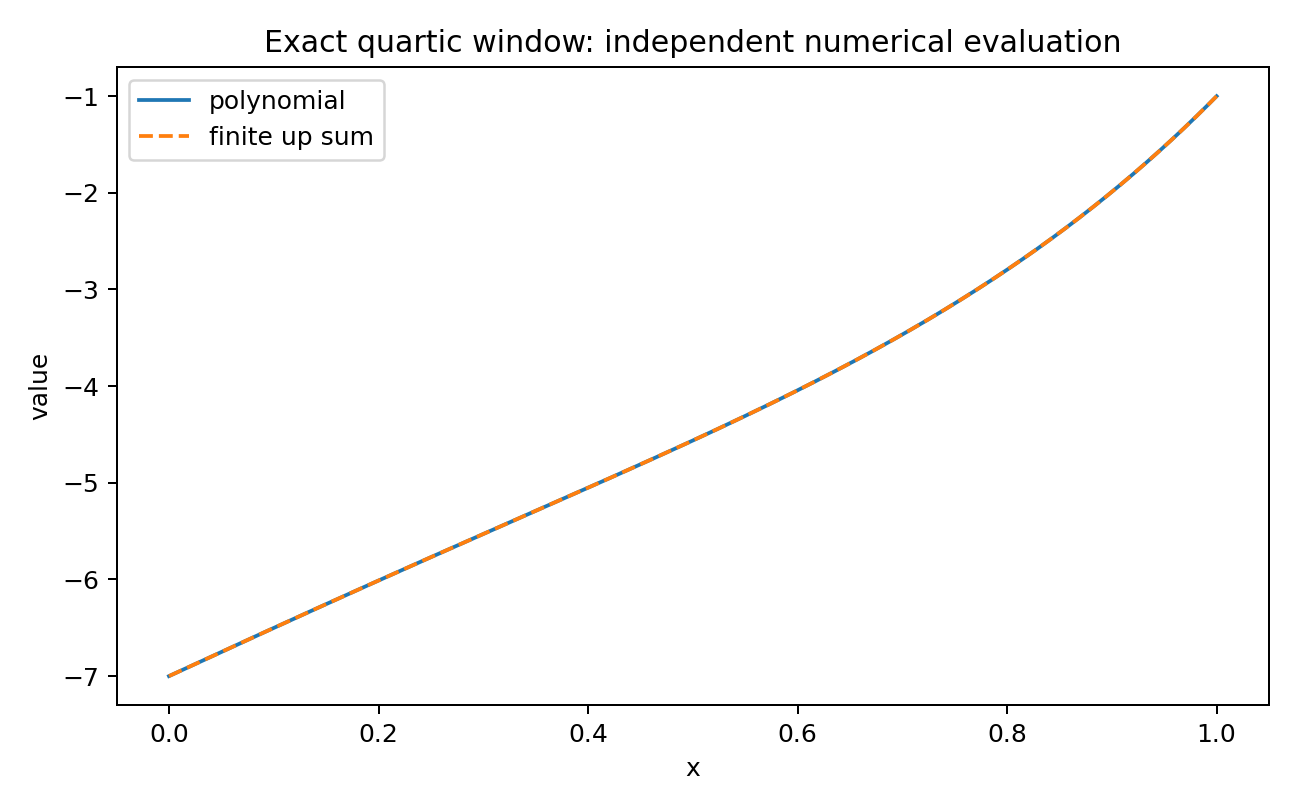
\includegraphics[width=0.88\textwidth]{generated/quartic_reconstruction.png}
\caption{The quartic and its finite ten-atom Rvachev-$u$ representation.  The
curves are visually indistinguishable.}
\label{fig:quartic}
\end{figure}

\begin{figure}[H]
\centering
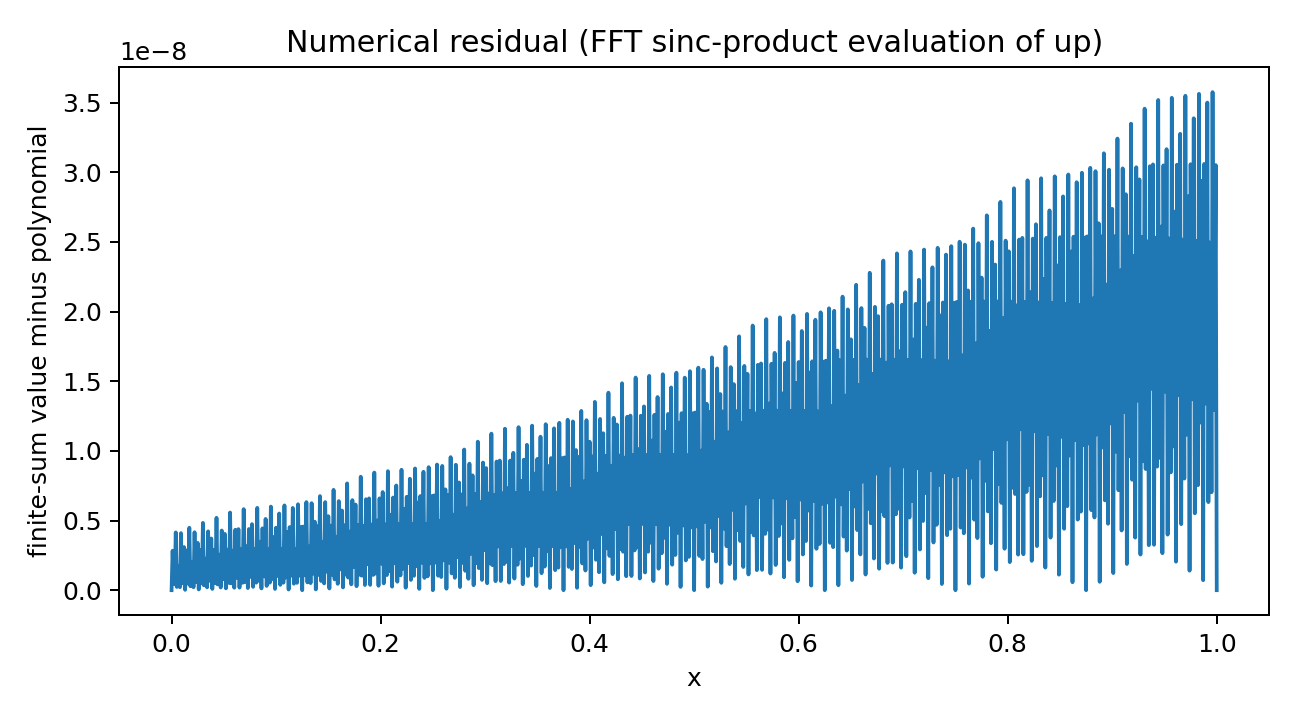
\includegraphics[width=0.88\textwidth]{generated/quartic_residual.png}
\caption{Residual from an independent FFT evaluation of the infinite sinc
product.  Exact symbolic verification gives zero.}
\label{fig:quartic-residual}
\end{figure}

\section{Numerical conditioning}

The sparse representation is algebraically simple but not automatically
well-conditioned in floating-point arithmetic.  Its level normalization is
\begin{equation}
 n!2^{n(n+1)/2},
 \label{eq:growth-normalization}
\end{equation}
which grows faster than exponentially.  The paired atoms are sampled near
increasingly flat portions of their large supports, so the polynomial emerges
from cancellation among large terms.  This is a familiar tension between exact
compact smoothness and numerical localization.

Recommended practice is:

\begin{itemize}
\item construct $b_n$ and $\alpha_{n,N}$ in exact rational arithmetic;
\item evaluate with extended or arbitrary precision for moderate or high $d$;
\item sum the atoms in equal-amplitude blocks, ordered by degree;
\item use compensated or pairwise summation;
\item reduce $h$ when a shorter support and smaller individual polynomial
  coefficients are worth the increased atom count;
\item optimize $h$ against an application-specific condition functional rather
  than choosing $h=L/2$ automatically.
\end{itemize}

The quasipolynomial estimate in \cref{prop:pm-quasi} explains why reducing $h$
does not simply make every coefficient worse.  As $K\sim L/(2h)$ grows, the
normalized binary weights behave like $N^n$, while the Appell coordinates of a
fixed polynomial carry powers of $h$.  There is substantial balancing, and a
nontrivial conditioning optimum should exist in many norms.

\section{Additional deductions}

\subsection{A reflected anticausal formula}

By symmetry, the right-tail operator
\begin{equation}
 (J_+f)(x)=\int_x^{\infty}f(t)\dd t
 \label{eq:Jplus}
\end{equation}
satisfies
\begin{equation}
 J_+u(x)=\sum_{k\geq0}u\!\left(\frac{x+(2k+1)}2\right).
 \label{eq:right-antiderivative}
\end{equation}
Iterating gives a mirror of \cref{thm:iterated-J}.  It yields exact polynomial
windows whose long support tail lies to the left instead of the right.  The two
orientations can be mixed degree by degree because any sequence of degree-$n$
monic polynomials remains a triangular basis.  This introduces a discrete
support-balancing design variable absent from the one-sided formula.

\subsection{Analytic-function approximation}

Let $f$ be analytic in a neighborhood of $[a,b]$.  Expanding
$\widetilde f(y)=f(c+hy)$ in the Appell basis and truncating at degree $d$ gives
an explicit finite $u$ sum.  Since $G(D)$ is an entire formal operator on
polynomials, the coefficients are computable from derivatives of $f$ at $c$.
Any standard polynomial approximation remainder immediately becomes a remainder
bound for finite $u$ sums.  Thus the exact polynomial theorem is also a direct
constructive approximation scheme for analytic and sufficiently smooth data.

\subsection{Tensor products}

On a box $I_1\times\cdots\times I_s$, tensor products of the univariate block
basis represent every multivariate polynomial exactly:
\begin{equation}
 \prod_{j=1}^{s}\Psi_{n_j}^{I_j}(x_j)
 \label{eq:tensor-basis}
\end{equation}
is a finite sum of tensor-product $u$ atoms.  A coordinatewise degree vector
$(d_1,\ldots,d_s)$ requires at most
$\prod_j2(d_j+1)$ raw tensor atoms in the direct sparse construction.  Low-rank
and total-degree compression are open optimization questions.

\subsection{Hermite jet stitching}

Because \eqref{eq:derivative-ladder} gives explicit endpoint derivatives, one
can solve finite Hermite systems to build compactly supported $C^\infty$
functions that agree with different prescribed polynomials on several disjoint
intervals.  The gaps carry smooth transitions automatically.  This offers a
new atomic-function analogue of polynomial splines with infinitely smooth
knots outside the exact polynomial plateaus.

\section{Conjectures and frontier problems}

The following statements are deliberately separated from the proved results.

\begin{conjecture}[Generic atom minimality in causal dyadic ladders
\Conjectural]
Fix $d$ and require a representation to use a single causal dyadic scale ladder,
with every degree block having a degree-independent left support edge and a
polynomial tail of exact degree $n$.  For a Zariski-open set of degree-$d$
polynomials, at least two atoms are necessary at every active level.  Hence the
canonical $2d+2$ count is minimal in this class.
\end{conjecture}

The restriction to a precise causal class is essential.  Global unrestricted
minimality is not claimed; nonlinear choices of centers and scales may permit
fewer atoms for special polynomials.

\begin{conjecture}[Support--atom Pareto optimality \Conjectural]
For fixed degree $d$ and collar size $\rho/L\to0$, any causal positive-scale
construction with uniformly controlled block condition number requires
$\Omega_d(L/\rho)$ atoms.  The bound in \eqref{eq:collar-count} is therefore
optimal up to a degree-dependent constant.
\end{conjecture}

\begin{conjecture}[Conditioning-optimal scale \Conjectural]
For every nonzero $p$ and interval $[a,b]$, natural coefficient and evaluation
condition functionals have at least one finite minimizer in $h>0$.  After
factoring the integer jumps of $K=\lceil L/(2h)\rceil$, the minimizer is unique
or belongs to a short finite set of adjacent $K$ regimes.
\end{conjecture}

\begin{conjecture}[$q$-ary refinable densities \Conjectural]
Let a compact density arise from a geometric random series with ratio $q^{-1}$,
$q\in\N$, and an appropriate uniform digit law.  Whenever its derivative
refinement has an integral translation stencil, repeated antiderivatives admit
weights generated by
\[
 \prod_{j=0}^{m-1}(1-z^{q^j})^{-1},
\]
and exact finite polynomial windows follow by the same support truncation.
The dyadic case is the most arithmetic because the reciprocal stencil is a
Thue--Morse block.
\end{conjecture}

\begin{problem}[Unrestricted minimal atom number]
Let $N_d$ be the smallest integer such that every real polynomial of degree at
most $d$ can be represented on every nondegenerate interval by at most $N_d$
shifted and positively scaled $u$ atoms with arbitrary real amplitudes.
Determine $N_d$.  This report proves
\[
 N_d\leq2d+2,
 \qquad N_0=2.
\]
Even $N_1$ appears to be a useful nontrivial test problem.
\end{problem}

\begin{problem}[Symmetric support optimization]
Combine causal and anticausal blocks, allowing degree-dependent orientation and
possibly unequal $h_n$, to minimize the maximum left/right collar subject to an
atom budget and a condition-number constraint.  Determine whether the
exponential one-sided scale growth can be reduced without increasing the atom
count above a linear function of $d$.
\end{problem}

\begin{problem}[Thue--Morse and $q$-binomial expansions]
Expand the Green weights $p_m(N)$ and their normalized versions $w_{n,N}$ in
bases adapted to Gaussian $q$-binomial coefficients, Prouhet cancellation, and
Mahler functional equations.  Seek identities that make the lower-order
quasipolynomial coefficients explicit and connect them to Bernoulli polynomials
on residue classes modulo $2^{m-1}$.
\end{problem}

\begin{problem}[Dual functionals and quadrature]
Construct compactly supported dual functionals $\lambda_n$ satisfying
$\lambda_n(\Psi_m)=\delta_{nm}$.  Determine whether they can be expressed by
finite dyadic samples or moments of $u$, and use them to derive exact quadrature
or local projection formulas.
\end{problem}

\begin{problem}[Formal verification]
A Lean formalization can be divided into four small modules:
\begin{enumerate}
\item the one-step telescoping identity;
\item the binary-partition induction;
\item the support-truncation theorem;
\item the finite-dimensional Appell operator inversion.
\end{enumerate}
None requires delicate asymptotic analysis, making the main theorem a promising
formalization target for the repository.
\end{problem}

\section{Implementation and reproducibility}

The archive accompanying this report contains
\begin{itemize}
\item \texttt{up\_polynomial\_representation.py}: exact construction,
  verification, and numerical sinc-product evaluation;
\item \texttt{generated/quartic\_atoms.csv}: the exact atom table;
\item \texttt{generated/quartic\_numerical\_check.csv}: 1001-point numerical
  comparison;
\item \texttt{generated/numerical\_summary.txt}: exact coefficients and error
  statistics;
\item the two figures used above.
\end{itemize}

A complete reproduction is obtained with
\begin{lstlisting}[style=pythonstyle]
python up_polynomial_representation.py --output-dir generated
\end{lstlisting}
The symbolic identity is independent of numerical evaluation.  The numerical
code computes the Fourier coefficients
\[
 \frac1P\widehat u\!\left(\frac{2\pi k}{P}\right)
\]
on a period $P=4>2$, truncates the infinite sinc product after 44 factors, and
uses an inverse FFT.  This is an independent check because the construction
uses the refinement/antiderivative identity while the numerical evaluator uses
the Fourier product.

\section{Conclusion}

The exact local polynomial-representation problem reduces to a surprisingly
rigid chain of inversions:

\begin{center}
refinement difference
$\longrightarrow$ antiderivative train
$\longrightarrow$ binary partitions
$\longrightarrow$ Appell polynomial tail
$\longrightarrow$ finite support truncation.
\end{center}

This chain yields an arbitrary-order algorithm with closed coefficients and no
numerical solve.  In its sparsest form, degree $d$ costs only $2d+2$ shifted and
scaled copies of one fixed $C^\infty$ compactly supported function.  In its
localized form, support collars can be prescribed at the cost of more atoms.
The same formulas expose a direct bridge among the Rvachev refinement equation,
the infinite sinc product, Bell--Bernoulli cumulants, restricted binary
partitions, and the signed Thue--Morse sequence.

Classical Rvachev theory already guarantees that suitable atomic-function
spaces contain polynomials.  The value of the present construction is its
explicitness: every center, scale, amplitude, support endpoint, determinant,
and arithmetic coefficient is available in closed form and can be verified in
exact rational arithmetic.  This makes the theorem suitable both for further
analysis and for formalization.

\appendix

\section{Detailed proof of the coefficient identities}

For completeness, we expand the operator calculation.  From
\eqref{eq:An-egf},
\[
 A_n(y)=\sum_{r=0}^{n}\binom nr\mu_r y^{n-r}=M(D)y^n.
\]
Suppose $\widetilde p=\sum_nb_nA_n$.  Since $G(t)M(t)=1$ as formal power
series,
\[
 G(D)\widetilde p
 =\sum_nb_nG(D)M(D)y^n
 =\sum_nb_ny^n.
\]
Now
\[
 G(D)\widetilde p(y)
 =\sum_{r=0}^{d}\gamma_r\frac{\widetilde p^{(r)}(y)}{r!}.
\]
Taking $n$ derivatives and evaluating at zero gives
\begin{align*}
 b_n
 &=\frac1{n!}\sum_{r=0}^{d-n}
   \frac{\gamma_r}{r!}\widetilde p^{(n+r)}(0)\\
 &=\sum_{r=0}^{d-n}
   \frac{\gamma_rh^{n+r}}{n!\,r!}p^{(n+r)}(c).
\end{align*}
If $\widetilde p=\sum_jc_jy^j$, then
\[
 [y^n]\frac{D^r}{r!}\widetilde p
 =\frac{(n+r)!}{n!r!}c_{n+r}
 =\binom{n+r}{r}c_{n+r},
\]
which proves \eqref{eq:b-coefficient}.

\section{Exact support bookkeeping}

For the general atom
\[
 u\!\left(
 \frac{x-a-h(2^{n+1}-2+2N)}{2^{n+1}h}
 \right),
\]
the center and radius are
\[
 C_{n,N}=a+h(2^{n+1}-2+2N),
 \qquad
 H_n=2^{n+1}h.
\]
Hence
\begin{align*}
 C_{n,N}-H_n&=a-2h+2hN,\\
 C_{n,N}+H_n&=a+h(2^{n+2}-2+2N).
\end{align*}
The minimum occurs at $N=0$ and the maximum at $(n,N)=(d,K)$, proving
\eqref{eq:support-total}.  Since $K< L/(2h)+1$,
\begin{align*}
 a+h(2^{d+2}-2+2K)
 &<a+h(2^{d+2}-2)+L+2h\\
 &=b+2^{d+2}h.
\end{align*}

\section{A compact table of exact formulas}

\begin{longtable}{@{}p{0.29\textwidth}p{0.66\textwidth}@{}}
\caption{Formula sheet for implementation.}\label{tab:formula-sheet}\\
\toprule
Object & Exact formula \\
\midrule
\endfirsthead
\toprule
Object & Exact formula \\
\midrule
\endhead
Cumulant & $\kappa_{2m}=2^{2m-1}B_{2m}/(m(2^{2m}-1))$, $\kappa_{2m+1}=0$.\\[0.4em]
Moment recurrence & $\mu_0=1$, $\mu_n=\sum_{r=1}^{n}\binom{n-1}{r-1}\kappa_r\mu_{n-r}$.\\[0.4em]
Reciprocal MGF & $G(t)=1/M(t)=\sum\gamma_rt^r/r!$.\\[0.4em]
$\gamma$ recurrence & $\gamma_0=1$, $\gamma_n=-\sum_{r=1}^{n}\binom{n-1}{r-1}\kappa_r\gamma_{n-r}$.\\[0.4em]
Appell polynomial & $A_n(y)=\sum_{r=0}^{n}\binom nr\mu_ry^{n-r}$.\\[0.4em]
Binary weight & $p_m(N)=[z^N]\prod_{j=0}^{m-1}(1-z^{2^j})^{-1}$.\\[0.4em]
Truncation index & $K=\lceil(b-a)/(2h)\rceil$.\\[0.4em]
Basis atom center & $C_{n,N}=a+h(2^{n+1}-2+2N)$.\\[0.4em]
Basis atom scale & $H_n=2^{n+1}h$.\\[0.4em]
Basis block & $\Psi_{n,h}=n!2^{n(n+1)/2}\sum_{N=0}^{K}p_{n+1}(N)u((x-C_{n,N})/H_n)$.\\[0.4em]
Polynomial coordinate & $b_n=\sum_{r=0}^{d-n}\gamma_rh^{n+r}p^{(n+r)}(a-h)/(n!r!)$.\\[0.4em]
Raw amplitude & $\alpha_{n,N}=n!2^{n(n+1)/2}b_np_{n+1}(N)$.\\[0.4em]
Support & $[a-2h,\;a+h(2^{d+2}-2+2K)]$.\\
\bottomrule
\end{longtable}

\section{Repository comparison checklist}

The following checks were used to avoid accidental duplication of the reviewed
corpus:

\begin{enumerate}
\item Search the representation syntheses for ``polynomial reproduction'',
``Strang--Fix'', ``finite polynomial'', ``binary partition'', and equivalent
variants.
\item Compare with the repeated-integration material, which studies convergence
of finite box-convolution iterates toward $u$ rather than inversion of the
refinement derivative into a polynomial tail.
\item Compare with the existing Appell sections, which organize dyadic Taylor
blocks of the Fabius function rather than interval-local sums of $u$ atoms.
\item Compare with the sinc-product and Fourier-zero sections, which supply the
MGF/Fourier data used here but not the support truncation.
\item Compare with the Thue--Morse and $q$-series drafts, where finite
Prouhet products occur but not as the discrete Green operator for repeated
antidifferentiation.
\item Check the historical/transcribed papers and, crucially, Rvachev's 1990
survey for classical polynomial-inclusion claims.
\end{enumerate}

The result is best viewed as a new synthesis and explicit constructive layer
built from known ingredients, not as a claim that the broad phenomenon of
polynomial representation by atomic functions was previously unknown.

\begin{thebibliography}{99}

\bibitem{Repository}
V.~Reshetnikov,
\emph{ProveIt: Analysis/FabiusFunction/docs}, recursive LaTeX research corpus,
GitHub repository, reviewed 28 August 2026.
\url{https://github.com/VladimirReshetnikov/ProveIt/tree/main/Analysis/FabiusFunction/docs}.

\bibitem{JessenWintner1935}
B.~Jessen and A.~Wintner,
``Distribution functions and the Riemann zeta function,''
\emph{Transactions of the American Mathematical Society} \textbf{38} (1935),
48--88.

\bibitem{Fabius1966}
J.~Fabius,
``A probabilistic example of a nowhere analytic $C^\infty$-function,''
\emph{Zeitschrift f\"ur Wahrscheinlichkeitstheorie und Verwandte Gebiete}
\textbf{5} (1966), 173--174.
\href{https://doi.org/10.1007/BF00536652}{doi:10.1007/BF00536652}.

\bibitem{Arias1982}
J.~Arias de Reyna,
``An infinitely differentiable function with compact support: definition and
properties,''
\emph{Revista de la Real Academia de Ciencias Exactas, F\'isicas y Naturales de
Madrid} \textbf{76} (1982), 21--38; reprint
\href{https://arxiv.org/abs/1702.05442}{arXiv:1702.05442}.

\bibitem{Arias2018}
J.~Arias de Reyna,
``Arithmetic of the Fabius function,''
\emph{Integers} \textbf{18} (2018), Article A51;
\href{https://arxiv.org/abs/1702.06487}{arXiv:1702.06487}.

\bibitem{RvachevRvachev1972}
V.~L. Rvachev and V.~A. Rvachev,
``On the representation of polynomials by functions with compact support,''
\emph{Mathematical Physics}, No.~11, Naukova Dumka, Kiev, 1972, 126--129.
MR~49 \#7406.  Bibliographic data as cited in \cite{Rvachev1990}.

\bibitem{Rvachev1977}
V.~A. Rvachev,
``On approximation by means of the function $\operatorname{up}(x)$,''
\emph{Doklady Akademii Nauk SSSR} \textbf{233} (1977), no.~2, 295--296
(Russian); English translation commonly cited in Soviet Mathematics Doklady.

\bibitem{Rvachev1990}
V.~A. Rvachev,
``Compactly supported solutions of functional-differential equations and their
applications,''
\emph{Russian Mathematical Surveys} \textbf{45} (1990), no.~1, 87--120.
\href{https://doi.org/10.1070/RM1990v045n01ABEH002324}{doi:10.1070/RM1990v045n01ABEH002324}.

\bibitem{StrangFix1973}
G.~Strang and G.~J. Fix,
\emph{An Analysis of the Finite Element Method},
Prentice--Hall, Englewood Cliffs, NJ, 1973.

\bibitem{deBoorRon1992}
C.~de Boor and A.~Ron,
``Fourier analysis of the approximation power of principal shift-invariant
spaces,''
\emph{Constructive Approximation} \textbf{8} (1992), 427--462.
\href{https://doi.org/10.1007/BF01203462}{doi:10.1007/BF01203462}.

\bibitem{deBoorDeVoreRon1994}
C.~de Boor, R.~A. DeVore, and A.~Ron,
``Approximation from shift-invariant subspaces of $L_2(\R^d)$,''
\emph{Transactions of the American Mathematical Society} \textbf{341} (1994),
787--806.

\bibitem{Roman1984}
S.~Roman,
\emph{The Umbral Calculus},
Pure and Applied Mathematics 111, Academic Press, New York, 1984.

\bibitem{Comtet1974}
L.~Comtet,
\emph{Advanced Combinatorics: The Art of Finite and Infinite Expansions},
Reidel, Dordrecht, 1974.

\bibitem{Andrews1998}
G.~E. Andrews,
\emph{The Theory of Partitions},
Cambridge Mathematical Library, Cambridge University Press, 1998 reprint.

\bibitem{AlloucheShallit2003}
J.-P. Allouche and J.~Shallit,
\emph{Automatic Sequences: Theory, Applications, Generalizations},
Cambridge University Press, 2003.

\end{thebibliography}

\end{document}
